\documentclass[a4paper]{article}
\usepackage{graphicx}
\usepackage{twocolpceurws}
\usepackage[utf8]{inputenc}
\usepackage{enumitem}
\usepackage{color}

\newcommand{\cn}[1]{\textsuperscript{\color{red} ~[citation needed](#1)~}}

\title{Measuring the degree of library dependency}

\author{
Núria Bruch Tàrrega \\ Universtiy of Amsterdam \\ nuria.bruchtarrega@student.uva.nl
\and
John X. Ceur \\ Science Dept.\\
                Online City, CEUR 99099 \\ jqq@ceur-ws.org
\and
Yvonne Onderzoeker \\ Research Dept.\\
                Science City, Sci 88088 \\ yvo@science.rdept.net
}

\institution{}




\begin{document}
\maketitle

\begin{abstract}
This is the abstract
\end{abstract}


\section{Introduction}
At present, there are many open-source libraries available for all developers to reuse the features that these libraries implement. This practice is becoming more and more popular since it allows to reuse previously developed code, and helps developers avoid implementing the same functionalities multiple times.

When a developer uses an open-source library in a project, it creates a dependency between the application and the library. This implies that a significant number of projects depend on other open-source projects, and it adds the task of managing these dependencies to the maintenance tasks of the project. How to maintain the dependencies is not a trivial task, and it is one of the problems that the field of software engineering is trying to solve \cite{kula2014visualizing}.

The management and maintenance of the dependencies of a project is an important task. Open-source libraries, just like any other software project, can have security vulnerabilities that may affect the projects that depend on these libraries. For example, some vulnerabilities can become security problems that can have a negative impact in terms of integrity, privacy or availability.

Currently, developers have at their disposal package managers, to ease the task of managing the dependencies of their projects. However, the dependency management available in these package managers only evaluate if a dependency exists or not and a more detailed risk evaluation is missing \cite{hejderup2018prazi}. There is no way to evaluate how much a project depends on a library.

Furthermore, it could happen that the developers of a project decide to replace one of the dependencies of the project with another one. This could happen in case a library has vulnerabilities or is deprecated, to prevent the vulnerabilities from affecting the project. However, replacing a dependency could be a costly process. It involves identifying which parts of the project are affected by the dependency, and which parts of the library are being used and need replacement.

Therefore, this thesis has the aim to perform a more detailed evaluation of the dependencies. A set of metrics is proposed to measure the dependencies between projects and the open-source libraries these use. In addition, we want to propose a way to measure the effort that would be required to replace a dependency with a new one. We are going to define a method to estimate effort considering which parts of the code are affected by the dependency.

\subsection{Research questions}
Based on the problem statement described, we define the following research questions:

\begin{itemize}[noitemsep]
  \item \textbf{RQ1:} \textit{How can we measure the degree of source code dependency between two libraries?}

  The goal of this research question is to define the metrics to measure a dependency. We focus on coupling metrics, which have been used for many years, in particular for Object-Oriented systems.

  \item \textbf{RQ2:} How can we measure the effort required to replace a dependency with another dependency with a different library?
\end{itemize}

\section{Background}\label{section:Background}
There are six main groups of coupling metrics \cite{poshyvanyk2006conceptual}: structural, dynamic, evolutionary and logical, information entropy approach, conceptual, and domain-specific. The most largely studied by the literature is the structural coupling, and it is the type of coupling measured in this research.

Briand et al. \cite{briand1999unified} defined a unified framework for coupling metrics, based on three previously existing frameworks. In their work, they specify are six criteria that define the type of coupling that a metric calculates. 1) The type of connection, which is the mechanism that creates coupling. 2) The locus of impact, or from which element of the relationship is the coupling being measured: the one that uses another element (import), or the one that is being used (export). 3) The granularity of the measure, which includes two aspects: the domain level (e.g. method, class, system), and how the metric counts the connections between the two elements (e.g. count each connection individually or binary evaluation of the connection between two elements). 4) The stability of the server, the server represents the element used by the other one in the relationship. The stability of the server is determined by the element being or not subject to modifications in the project at hand. 5) Direct/Indirect coupling, if the metric accounts for indirect relationships, or only measures the direct ones. 6) Inheritance, this criterion specifies how certain special cases (e.g. inheritance and polymorphism) affect the coupling between two elements.

\section{Related Work}
Soto-Valero et al. \cite{soto2020comprehensive} conducted a study of bloated dependencies. Bloated dependencies are included in the dependency set of a project, either direct or transitive, but there is no real dependency since the libraries are unused. They developed the tool \textit{DepClean}, which analyses the dependencies of Java artifacts, to define which are bloated and to generate an alternative dependency file without bloated dependencies. Pashchenko et al. \cite{pashchenko2018vulnerable} propose a method to analyze dependencies in which they distinguish between own and third-party libraries, as well as deployed and non-deployed dependencies. In addition, they remark the increased risk related to halted dependencies, since the libraries related to these dependencies are not updated.

Hejderup et al. \cite{hejderup2018software} propose a technique to represent software ecosystems at a function level, a versioned call based dependency network. This call-level dependency graph, in contrast with a package-level dependency graph, allows performing a more detailed evaluation of the dependencies. The graph is used to analyze how the bugs and vulnerabilities spread across the dependency network. In another study Hejderup et al. \cite{hejderup2018prazi} define an approach, named Präzi, to generate call-level dependency networks. In particular, they implement this approach for the Rust ecosystem and discuss all the perils affecting the soundness and precision of Präzi. They conclude that RustPräzi is three times more precise than the package-level dependency graphs.

\section{Dependency evaluation model}
The first steps towards a creating a model to measure the dependencies between libraries is to define which meaning of coupling is involved in these depenencies. Therefore, we will use the framework explained in section \ref{section:Background}, from Briand et al. \cite{briand1999unified}. When deciding about the 6 criteria specified in the framework, the order of the decisions is important, since some criteria may directly discard some options of other criteria. Hence, we are going to start by those criteria that are clearly defined by the problem statement.

\paragraph{Criterion 2: Locus of impact}
According to the description of the problem, the goal of this measurement is to know how much a library depends on another. Therefore, the point of view of this evaluation is from the library that uses another one. Hence, the locus of impact of the coupling to be measured in this thesis is \textbf{import}.

\paragraph{Criterion 4: Stability of the server}
Briand et al. \cite{briand1999unified} define stable classes as \textit{"Classes that are not subject to change in the project at hand"}. Therefore, we are going to measure coupling from non-stable classes to stable classes.
However, the separation between stable and unstable classes is not enough. The goal is not to measure the coupling with all stable classes since these include classes such as types provided by the programming language and standard libraries. Therefore, the coupling will only be measured with \textbf{stable classes} that are part of other third-party open-source libraries.

\paragraph{Criterion 5: Direct and indirect coupling}
To decide which option we want to define for this criterion, we need to distinguish two alternative scenarios in which we want to measure coupling: Direct dependencies and transitive dependencies. For the initial approach, we are going to focus on the direct dependencies only. Therefore, the metrics are going to measure \textbf{direct coupling} only. However, the metrics defined to measure direct coupling can be extended to consider indirect coupling.

\paragraph{Criterion 3: Granularity of the measure}
In this criterion, there are two aspects to define. The domain level of the measure, and how the metric counts the connections. First, we are going to discuss the domain level. Briand et al. define the following levels:

\begin{itemize}[noitemsep]
  \item Attribute
  \item Method
  \item Class
  \item Set of classes
  \item System
\end{itemize}

In this case, the goal is to measure the coupling between the set of classes of the client library and the set of classes of the server library. However, in order to maintain consistency, we rename the domain level set of classes as \textbf{library} for the rest of the paper. To maintain the precision of the measurement, the calculation of coupling for a more coarse-grained level, such as library, is done by aggregating the coupling of the more fine-grained domains.

Next, we define how the metrics count the connections. The options for counting connections defined in the framework, are based on two options for the domain levels method and attribute: counting individual connections (option A), and count the items at the other end of the connection (option B). Since the goal is to measure the degree of dependency, we need to focus on option A, since it counts the number of connections. Based on option A, Briand et al. define option C: "Add up the number of connections counted as in A) for each method or attribute of the class". Based on option C, we define the following option for counting connections at the library level: \textbf{Add up the number of connections counted as in C) for each class of the library}.

\paragraph{Criterion 1: Type of connection}
With this criterion, it is defined which type of connection creates coupling between the two items, the two libraries. There are several and clearly distinguished mechanisms that can create coupling \cite{briand1999unified}, listed below.

Given class \textit{a} that belongs to library \textit{A}, and class \textit{b} that belongs to library \textit{B}...

\begin{enumerate}[noitemsep,leftmargin=*]
  \item ... class \textit{a} has an attribute of type \textit{b} (Relationship of aggregation).
  \item ... method of class \textit{a} has a parameter of type \textit{b} or has return type \textit{b}.
  \item ... method of class \textit{a} has a local variable of type \textit{b}.
  \item ... method of class \textit{a} calls a method which has a parameter of type \textit{b}.
  \item ... method of class \textit{a} references attribute of class \textit{b}.
  \item ... method of class \textit{a} invokes method of class \textit{b}.
  \item ... class \textit{a} and class \textit{b} have a relationship such as \textit{uses} or \textit{consists-of}.
\end{enumerate}

Having one metric measure more than one of these types of connections is not recommended. To begin with, the strengths of every type of connection have to be justified: Has one connection of type 5 the same strength as a connection of type 6? Also, it is not possible to know how much of the coupling is created by which type of connection. Therefore, all chosen types of connections are going to be measured by different metrics. To decide which types of connections to measure, since all of them create coupling between libraries, we have decided to review the literature on coupling metrics, to understand which connections are the most measured and why.

THIS IS A HUGE TODO

\paragraph{Criterion 6: Inheritance (Special cases)}
Within this criterion, there are three aspects to decide about: how, if at all, does the metric distinguish between inheritance-based coupling and noninheritance-based coupling? If the metric counts method invocations, does it account for polymorphism? And finally, what defines if a method or attribute is part of a class or not? This questions are going to be discussed and answered by using Figure \ref{fig:specialcases}, based on the work from Briand et al. \cite{briand1999unified}.

\begin{figure}[ht]
\begin{center}
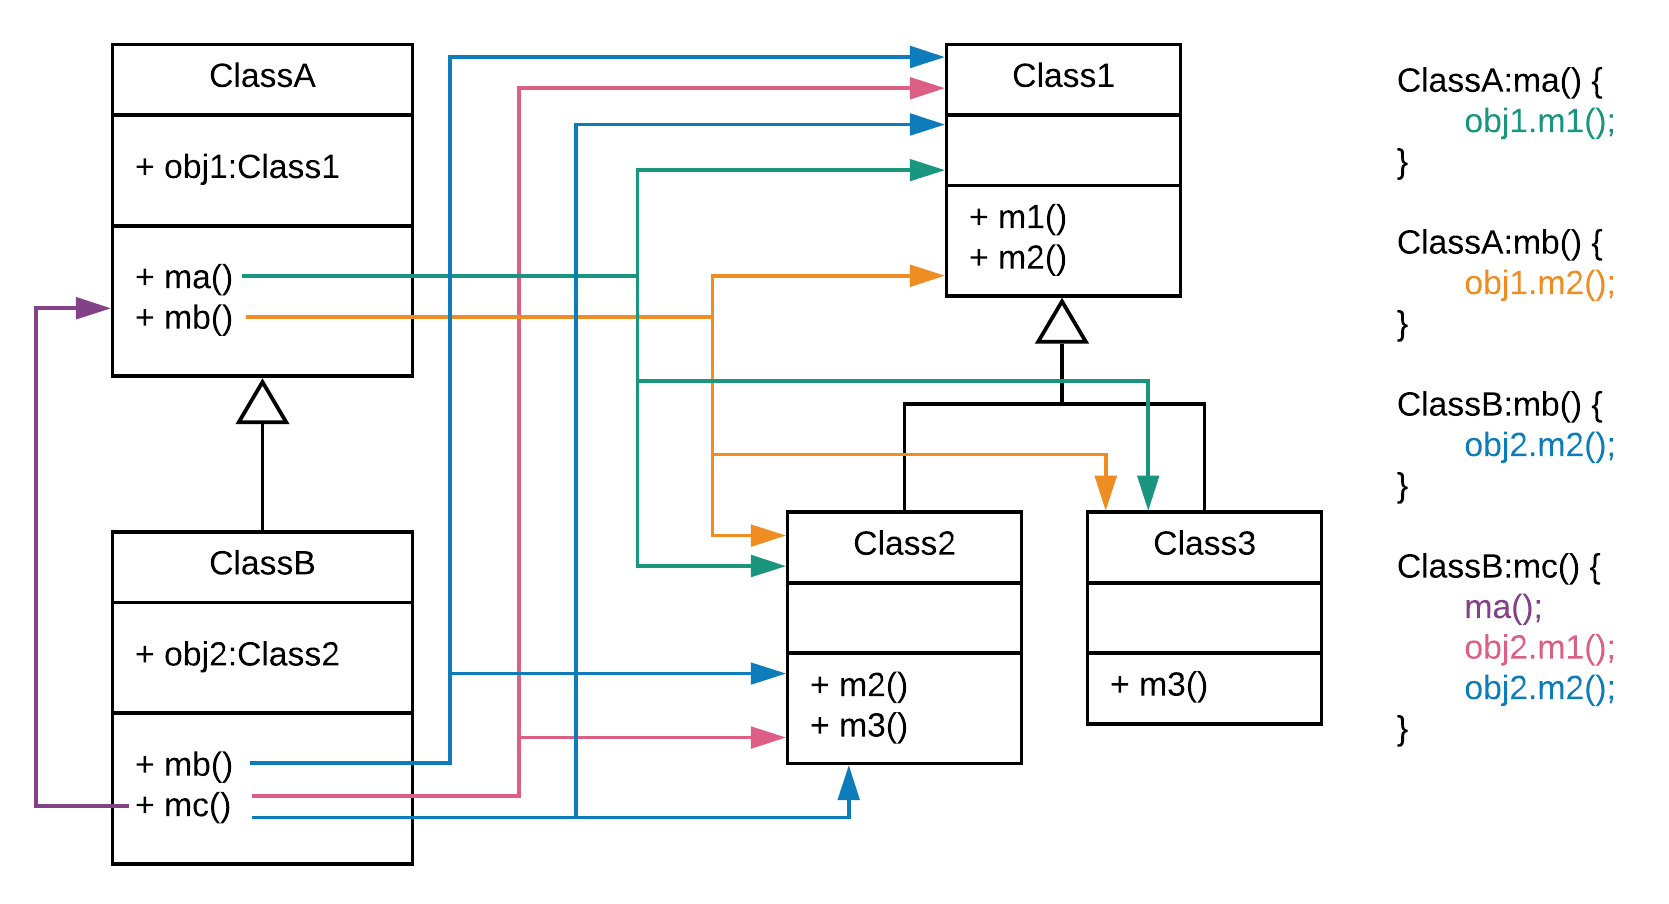
\includegraphics[height=4.5cm]{img/specialcases.png}
\caption{Example of coupling special cases}
\label{fig:specialcases}
\end{center}
\end{figure}

In Figure \ref{fig:specialcases}, the method \texttt{mc} of \texttt{ClassB} calls the method \texttt{ma} of \texttt{ClassA}. Since \texttt{ClassB} inherits from \texttt{ClassA}, this is known as inheritance-based coupling. In the case that the two involved classes where part of different libraries, this connection would create coupling between the libraries. However, should this connection be considered as a special case and count it separatedly from the rest? To answer this question, we look at it from the point of view of our problem statement: Is it more or less dificult to maintain inheritance-based coupling than non-inheritance-based coupling? The answer is no, if there is a change in an inherited method that a class is using, it will require the same maintenance effort than in the case the method is not inherited. Therefore, our metrics are going to \textbf{include inheritance-based coupling without distinction}.

The next line of the same method, makes a call to \texttt{m1}, from an object of type \texttt{Class2}. However, this method is not implemented in \texttt{Class2}, but in \texttt{Class1}. With which classes does this call create coupling? From a maintenance perspective, if the method is updated in \texttt{Class1}, this will probably require updates in \texttt{ClassB} as well. Furthermore, if \texttt{Class2} is \cn{HELLO DO THIS}

The last line of \texttt{mc} calls the method \texttt{m2} from an object of type \texttt{Class2}. This method, inherited from \texttt{Class1}, is overridden in \texttt{Class2}. Therefore, this creates coupling with \texttt{Class2}, but does it create coupling with \texttt{Class1}? \cn{HELLO DO THIS}

Then, if we focus on the method \texttt{ma} of \texttt{ClassA}, we see that it calls \texttt{m1} in an object of type \texttt{Class1}. However, the dynamic assignation of types, can make this object be of type \texttt{Class2} and \texttt{Class3}. Does this method call create coupling with \texttt{Class2} and \texttt{Class3}? \cn{HELLO DO THIS}.

Finally, a similar case happens with method \texttt{mb}, the difference is that in this case it calls \texttt{m2}, which in \texttt{Class2} is overridden. Does this create coupling with \texttt{Class2}? In other words, do we account for all possible polymorphic method invocations? If we consider the case in which the implementation of \texttt{m2} in \texttt{Class2} changes, this may affect the way \texttt{ClassA} uses it, and therefore changes may be needed. Thus, we consider that it is necessary to \textbf{account for polymorphism}.

\section{Formal definition of the metrics}

\subsection{Metric 1: Method invocation coupling}
\[
  MIC(L, L') = \sum_{c \in C(L)}^{} \sum_{m \in M(c)}^{} indMI(m, L')
\]

\[
  indMI(m, L') = \sum_{m' \in SIM(m)}^{} NI(m, m')*PM(m', L')
\]

C(L) --- Classes of library \textit{L}

M(c) --- Methods implemented in class \textit{c}

SIM(m) --- Set of stable methods invoked in \textit{m}

NI(m, m') --- Number of invokations of \textit{m'} in \textit{m}

PM(m', L') --- Number of polymorphic methods of \textit{m'} implemented in library \textit{L'}

\subsection{Metric 2: Aggregation coupling}
\[
  AC(L,L') = \sum_{c \in C(L)}^{} \sum_{c' \in AT(c)}^{} NA(c, c')*DC(c', L')
\]

AT(c) --- Set of stable attribute types of class \textit{c}.

NA(c, c') --- Number of attributes of type \textit{c'} in class \textit{c}.

\section{Evaluation Setup}
% We are going to develop a proof-of-concept tool in order to calculate the proposed metrics to measure the dependencies. In this tool, the metrics are going to be calculated from call-level dependency graphs, which will contain the dependency network of the evaluated library.


\section{Preliminary Results}



\section{Conclusion}

\subsection{Next steps}


\bibliographystyle{alpha}
\bibliography{res}
%inline the .bbl file directly for mailing to authors.

\end{document}
